\chapter{Theory}
% Hier folgt eine kurze Einleitung in die Thematik der Bachelorarbeit.
% Die Einleitung muss kurz sein, damit die vorgegebene Gesamtlänge der 
% Arbeit von 25 Seiten nicht überschritten wird. 
% Die Beschränkung der Seitenzahl sollte man ernst nehmen,
% da Überschreitung zu Abzügen in der Note führen kann. 
% Um der Längenbeschränkung zu genügen, darf auch nicht an der Schriftgröße,
% dem Zeilenabstand oder dem Satzspiegel (bedruckte Fläche der Seite) manipuliert werden.


The IceCube neutrino detector is a cubic kilometer scale particle detector located near the Amundsen-Scott South Pole Station. The primary goal of 
the detector is the detection of high energy neutrinos as messenger particles for study of astrophysical sources. The detector unit is split into three 
parts, which are the In-Ice Array, the IceTop, and the DeepCore. 

The In-Ice Array is the largest component and consists of 86 vertical strings, extending vertically into the ice below the surface for \SI{2450}{\metre}. 
Each of the strings contains 60 Digital Optical Modules (DOMs) starting from a depth of \SI{1450}{\metre} all the way down to \SI{2450}{\metre}
The DOMs are evenly separated by \SI{17}{\metre} alongside their respective string, making a total number of \num{5160} DOMs. 

The IceTop, as the name suggests, is located at the surface of the ice with \num{162} tanks filled with ice and equipped with PMTs. 
The tanks are arranged in 81 stations in a manner that approximately mimics the structure of the In-Ice Array. 

The DeepCore is a sub-array within the In-Ice Array and is located at depths beneath \SI{1750}{\metre}. It contains an extra \num{8} strings alongside the 
\num{7} strings from the In-Ice Array. This creates a more densly packed arrangement of DOMs in the lower center of the detector, which increases its 
ability to detect low-energy signals.

Figure~\ref{fig:icecube_sketch_01} shows a visual representation of this structure.

\begin{figure}[htbp]
    \centering
    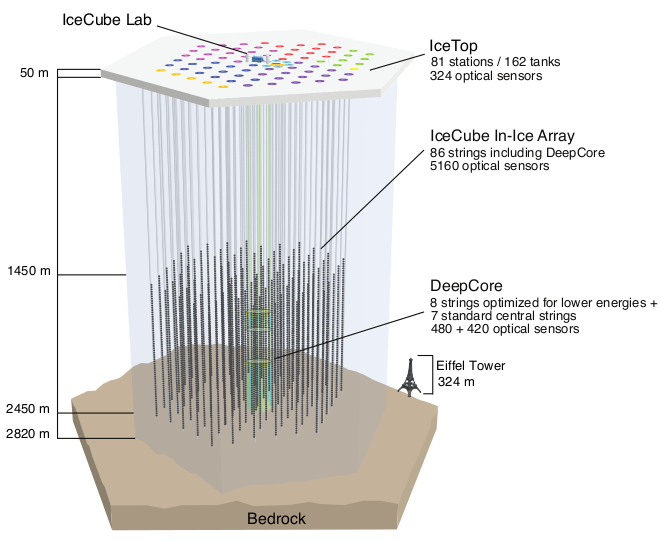
\includegraphics[width=\textwidth]{content/pictures/icecube_sketch_01.png}
    \caption{An overview of the arrangement inside of the detector.}\label{fig:icecube_sketch_01}
\end{figure}

\section{Digital Optical Module}

A single DOM consists of a glass housing, in which the PMT and the corresponding curcuit boards are located. The technical part of the functionality of 
the circuit boards are not of interest for this analysis, so I will not go into detail on that topic. The PMT however is the actual detecting unit of 
the DOM\. A sketch of a PMT is shown in figure~\ref{fig:pmt01}.

\begin{figure}[htbp]
    \centering
    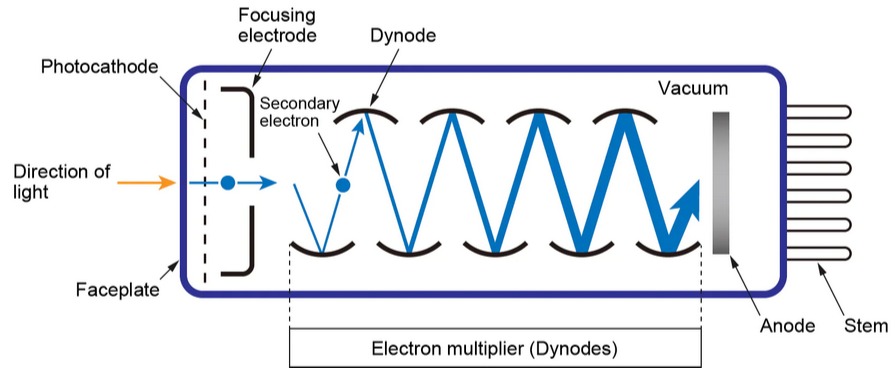
\includegraphics[width=\textwidth]{content/pictures/pmt_sketch_01.png}
    \caption{The principle construction of a photomultiplier.}\label{fig:pmt01}
\end{figure}

When a photon with sufficient energy hits the photocathode of the PMT, its energy gets absorbed and an electron is emitted via the photoelectric effect.
the electron is accelerated towards the first dynode due to its electric charge. Hitting the dynode triggers secondary emittions, increasing the total 
number of electrons emitted. This process repeats itself for however many dynodes are the PMT accompasses. After the final amplification by the last 
dynode the electrons are collected by the anode, which produces a current proportional to the intensity of the initial light signal, meaning the amount of
photons hitting the PMT\@. 

\section{Cherenkov radiation}

The light detected by the photomultipliers is only a secondary signal called Cherenkov radiation. It is created when a charged particle travels through a 
dielectric medium with a velocity greater than the speed of light inside of the medium. The charged particle polarizes the medium's molecules in its
immediate surroundings while passing through it. The excited molecules then return to their ground state by emitting their superfluous energy as light.
Because the light travels slower than the particle exciting the molecules, the light waves do not interfere destructively, but build a conical shock front 
similar in principle to that of an object, moving through air at supersonic velocities. This cone of light is the Cherenkov radiation detected by the PMTs.

\section{Muons}

A significant percentile of the particles measured in IceCube are muons, which are elementary particles categorized as leptons by the standard model.
This means they carry an electric charge of $\pm 1e$ and have spin $\frac{1}{2}$. The mass of the muon is \num{105.658}\text{MeV}. IceCube detects
muons at a rate of roughly \SI{2500}{Hz}. While they are muons originating from outer space that hit the earths surface, the vast majority of muons detected
on earth are created in the atmosphere. When cosmic rays collide with the atmosphere's molecules, a multitude of secondary particles are created including 
pions and kaons. The average lifetime of these mesons are of the magnitude of \SI{e8}{s} or less. Their resulting decay products include muons which are 
produced via the following decay modes:\\

\begin{align}
    \pi^\pm \to \mu^\pm + \nu_\mu \\
    K^\pm \to \mu^\pm + \nu_\mu
\end{align}

These muons have an average lifetime of about \SI{2.2}{ms}, which is enough for a significant amount of them reaching the earths surface due the their 
ultrarelativistic velocities. When a muon travels through the ice within IceCube, it produces Cherenkov radiation due to its charge and high velocities and 
can thus be indirectly measured.

\section{Data aquisition}\label{sec:daq}

A single DOM measureing a signal is not able to distinguish between different types of events, since its only capability lies in the detection of a current
caused by photons hitting the PMT\@. In order to distinguish between noise and possible signals stemming from Cherenkov radiation, multiple requirements are
put in place to ensure that the full data of a signal is only saved for those signals that might constitute a real event. The data aquisition systems (DAQ)
is the software complex responsible for filtering signals by different characteristics. The first step for any signal is to scan for so called hard local 
coincidences (HLC). 
There are so called triggers implemented which search for multiplicities of HLC hits within a certain time frame and with certain spatial requirements.
The simplest one is the simple multiplicity trigger (SMT), which triggers whenever at least $N$ HLC hits occur within a time frame of some 
\si{\micro\second}. This sets a set of intuitive conditions for grouping a cluster of signals into an event that could be a muon or another 
charged particle emitting Cherenkov radiation. 
Another trigger is the fixed rate trigger (FRT) which is of great importance for the analysis of this thesis. The FRT does not get triggered 
by any multiplicity of events. It is a timed trigger which reads out the entire detector, meaning all functioning DOMs for \SI{10}{ms}
every \SI{300}{s}. Since there are no conditions of any kind in place for this trigger, it saves everything being measured during the 
readout time frame. This allows a precise look into the low energy spectrum of signals hitting the detector which is significant for the 
analysis of the backround noise in IceCube. An overview of different triggers, which are not primarily significant for this thesis is shown 
in figure~\ref{fig:triggers}.

\begin{figure}[htbp]
    \centering
    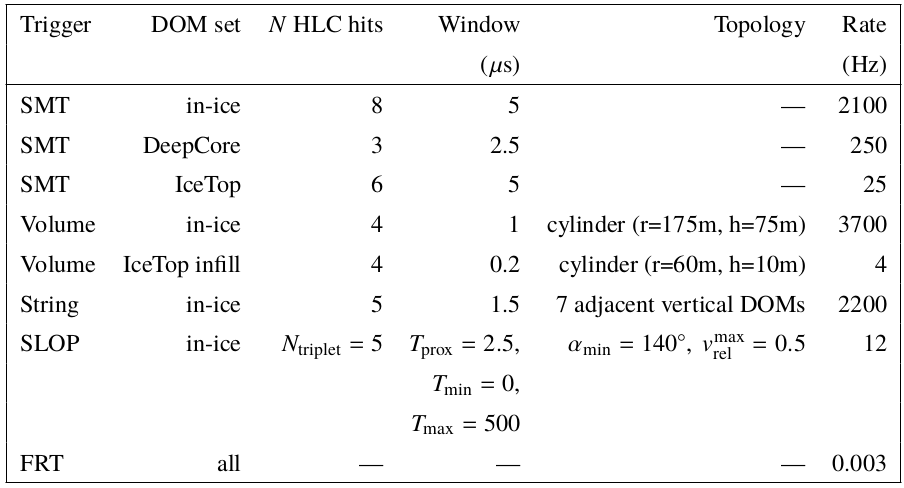
\includegraphics[width=\textwidth]{content/pictures/trigger_list.png}
    \caption{A list of all triggers in IceCube.}\label{fig:triggers}
\end{figure}

\section{True coincident events}

The primary goal of this thesis is the analysis of coincident events in IceCube. This is not to be confused with coincident signals or hits, which are used 
to determine if an event is constituted by the signals. A coincident however means that two or more real events take place in the detector within the time 
frame of a readout window from some trigger. The SMT for example will group together any multiplicity of HLC hits in the detector and categorize them as one
event, as long as no other measures are taken. The resulting events would falsely be forwarded as one which leads to the loss of information aswell as 
a count rate of events in the long run. \\
Firstly, a rough estimation can be made about the percentile of coincident events for any given event rate. A single particle type's spectrum can be 
estimated to be poisson distributed, so probability to measure $k$ events becomes\\ 

\begin{equation}
    P_{\lambda}(k) = \frac{\lambda^k}{k!}\text{e}^(-\lambda) \; .
\end{equation}\\

$\lambda$ is the expected value, which can be rewritten as \\

\begin{equation}
    \lambda = R \cdot \tau \; ,
\end{equation}\\

where $R$ is the rate of incoming particles and $\tau$ is the search time frame set by the trigger, as explained in section\.~\ref{sec:daq}. 
The value of interest is the probability for 2 or more particles hitting the detector within a certain time frame. This would be \\

\begin{equation}
    P_{\lambda = R\cdot\tau}(k\geq2) = e^{- R\cdot\tau} \cdot \sum_{k=2}^\infty \frac{{(R\cdot\tau)}^k}{k!} \; .
\end{equation}\\ 

Multiplying with the event rate $R$ then yields the coincidence rate $R_{co}$ depending on the event rate and the readout window $\tau$:

\begin{equation}
    R_{co}(R,\tau) = R \cdot e^{- R\cdot\tau} \cdot \sum_{k=2}^\infty \frac{{(R\cdot\tau)}^k}{k!}\;.
\end{equation}\\

\section{Fixed Rate Trigger}

The FRT, as explained in section\@~\ref{sec:daq}, holds a speical significance for the analysis of coincident events in IceCube. 
Analyzing the signals collected by the FRT opens a window into the unfiltered distribution of signals collected by the detector. 
As the FRT's data does not undergo any data reduction, it includes all backround noise aswell as all other low energy 

